\documentclass[11pt, oneside]{article}   	% use "amsart" instead of "article" for AMSLaTeX format
\usepackage{geometry}                		% See geometry.pdf to learn the layout options. There are lots.
\geometry{letterpaper}                   		% ... or a4paper or a5paper or ... 
%\geometry{landscape}                		% Activate for for rotated page geometry
%\usepackage[parfill]{parskip}    		% Activate to begin paragraphs with an empty line rather than an indent
\usepackage{graphicx}				% Use pdf, png, jpg, or eps§ with pdflatex; use eps in DVI mode
								% TeX will automatically convert eps --> pdf in pdflatex		
\usepackage{amssymb}

\title{Calibrated, Parametrized Learning}
\author{Kyle Cranmer and Daniel Whiteson}
%\date{}							% Activate to display a given date or no date

\begin{document}
\maketitle

\section{Introduction}
%\subsection{}


Notation:

\begin{itemize}
 \item $x$: a vector of observed quantities for each event (energy, momenta, angles of particles)
 \item $D$: a dataset of $D=\{x_1, \dots, x_n\}$
 \item $\theta$: parameters of a statistical model
\item $f_c(x| \theta)$:  probability density function (statistical model) for $x$ for category $c\in\{0,1\}$.
\item $s(x)$: real-valued score from a machine learning classification algorithm (or any map $s: X\to\mathbb{R}$)
\item $s(x;\theta)$: real-valued score from a parametrized machine learning classification algorithm (or any map $s: X\otimes \Theta \to\mathbb{R}$)
\item $f_c( s | \theta )$ The probability density function for $s$ implied by $f_c(x|\theta)$ and $s(x)$
\item $f_c( s(\cdot; \theta) | \theta )$ The probability density function for $s$ implied by $f_c(x|\theta)$ and $s(x;\theta)$

\end{itemize}

\subsection{Typical usage of machine learning in HEP}

In high-energy physics (HEP) we typically are searching for or measuring the properties of some 
class of events, generically referred to as \textit{signal}, in the presence of a separate class 
of \textit{background} events. For each event we measure some quantities $x$ that have corresponding distributions 
$f_0(x|\theta)$ for background and $f_1(x|\theta)$ for signal.  Often machine learning classification algorithms are trained on large samples of synthetic data $\{x_i, c_i\}$ generated with some nominal values of the parameters $\theta_0$, where $c=0$ corresponds to background and $c=1$ corresponds to signal. The resulting classifier is denoted $s(x)$. Based on this classifier and large samples of synthetic data drawn from $f_c(x | \theta)$ we construct the distribution  $f_c(s | \theta)$. An example of the distributions of the distribution of $s$ for the signal and background events with $\theta=\theta_0$ is shown in Figure~\ref{fig:tmva}.


\begin{figure}[htbp]
\begin{center}
 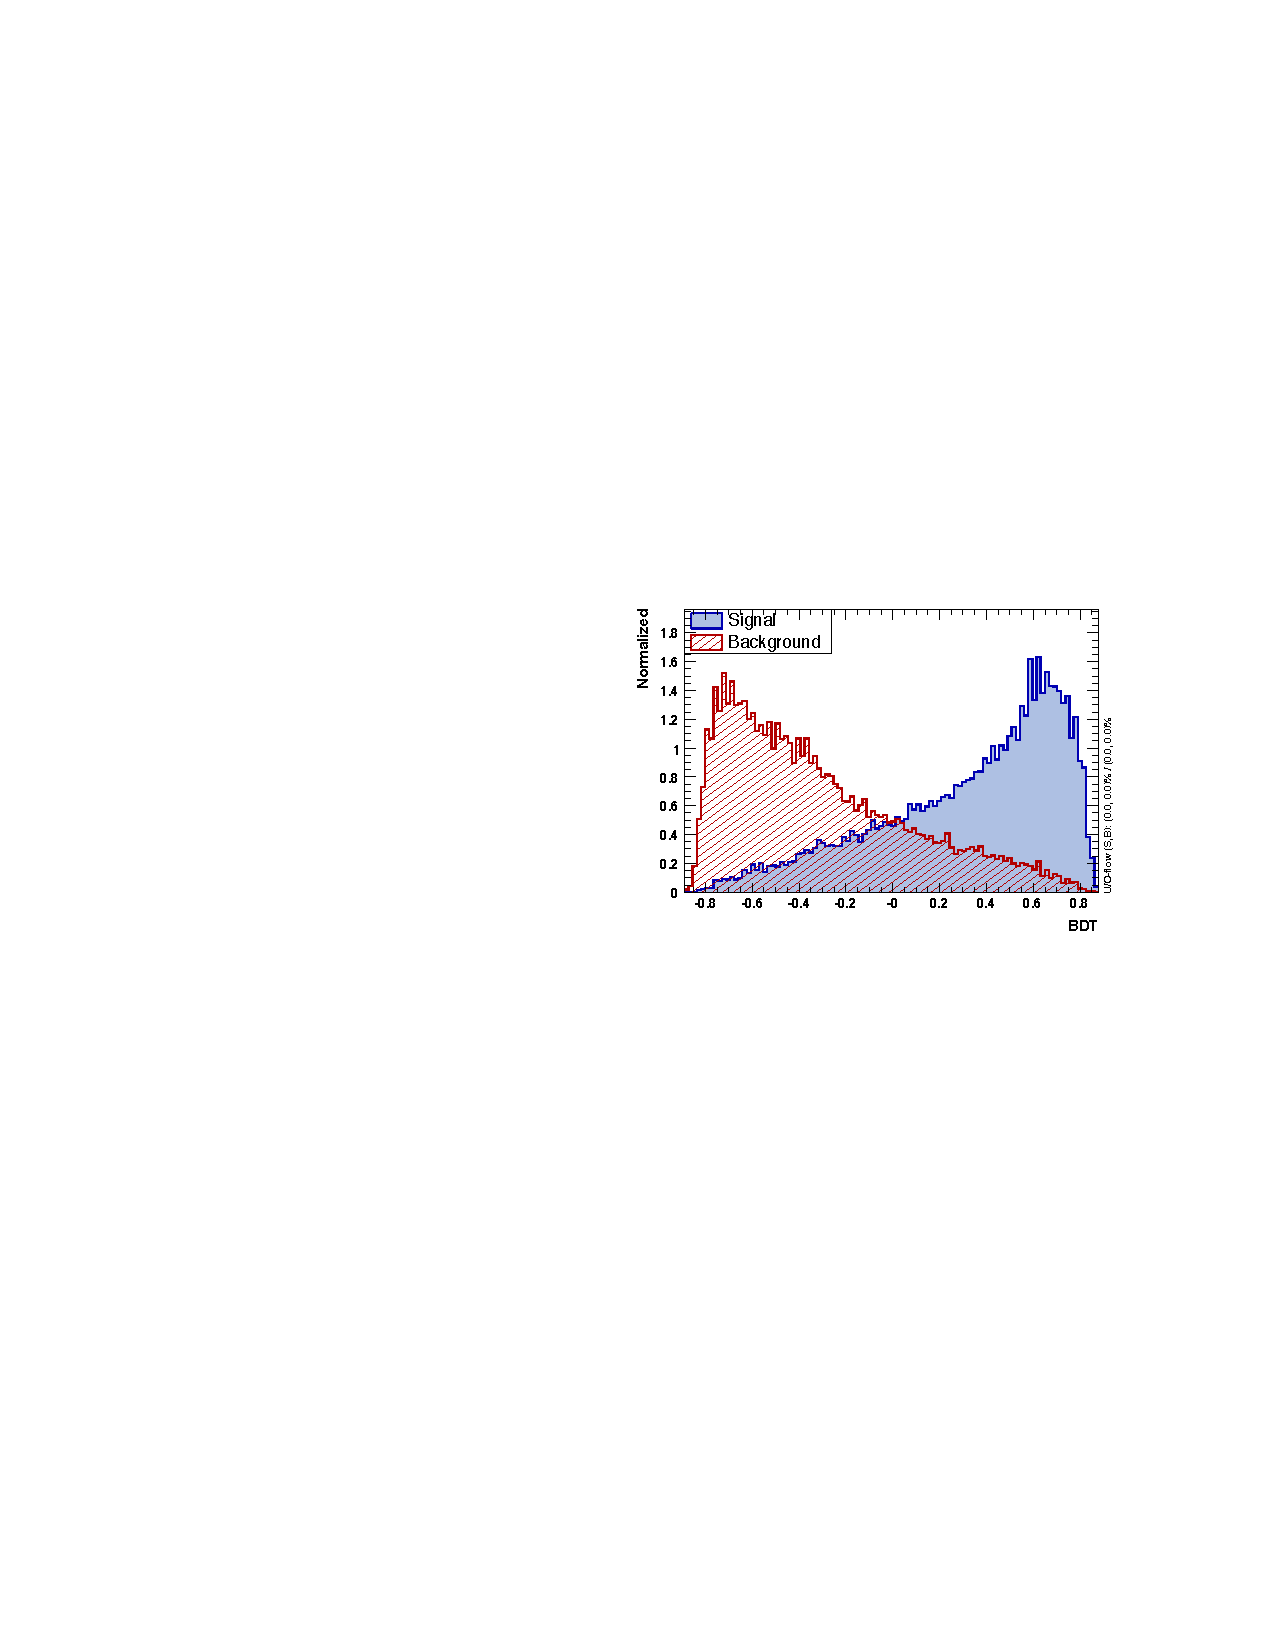
\includegraphics[height=2in]{example-TMVA-BDT.pdf}
 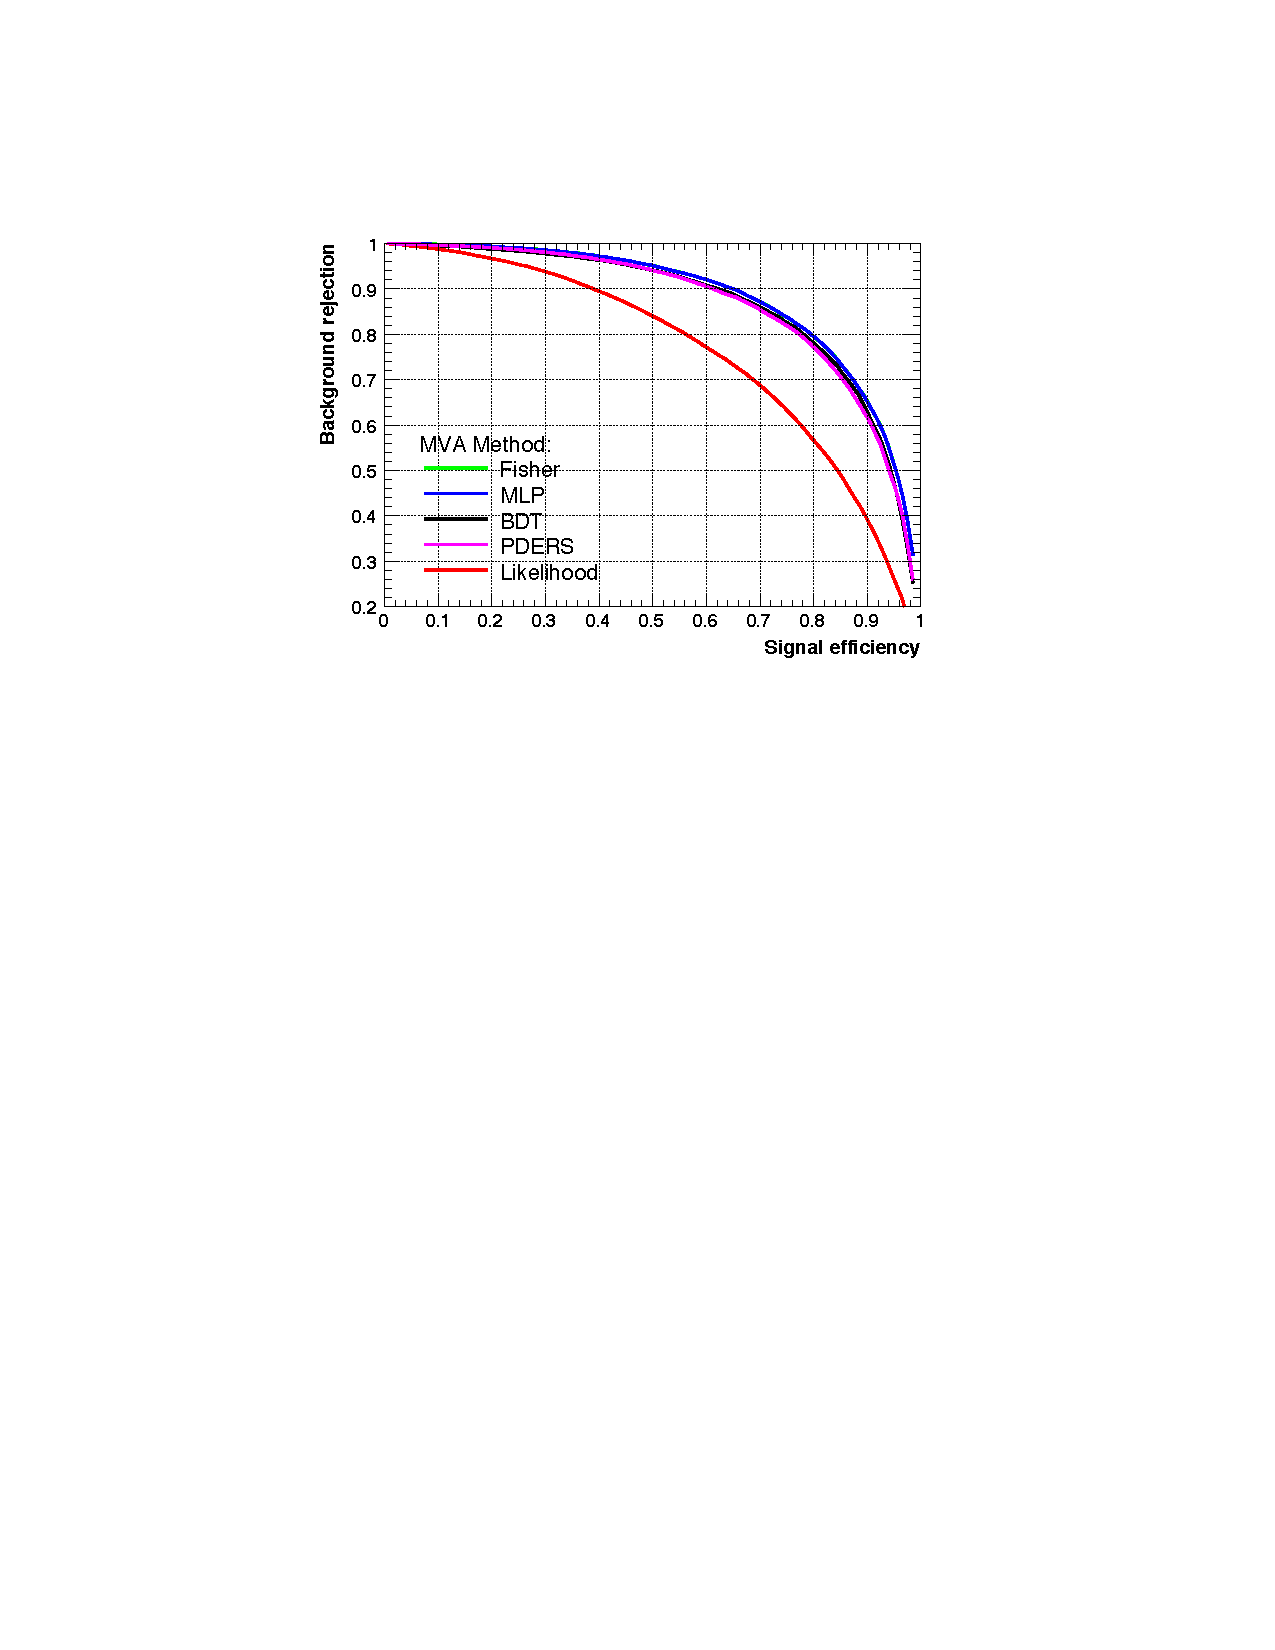
\includegraphics[height=2in]{example-TMVA-ROC.pdf}
\caption{Left: an example of the distributions $f_0(s|\theta)$ and $f_1(s|\theta)$ when the classifier $s$ is a boosted-decision tree (BDT). Right: the corresponding ROC curve (right) for this and other classifiers. Figures taken from TMVA manual.}
\label{fig:tmva}
\end{center}
\end{figure}

These steps lead to a subsequent statistical analysis where one observes in data $\{x_e\}$, where $e$ is an event index running from $1$ to $n$. For each event, the classifier is evaluated and one performs inference on a parameter $\mu$ related to the presence of the signal contribution. In particular, one forms the statistical model
\begin{equation}\label{eq:typicalML}
f( D \,|\, \mu, \theta) = \prod_{e=1}^n \, \left[\, \mu f_1( s(x_e) \, |\,  \theta)  + (1-\mu)\, f_0( s(x_e) \,|\, \theta) \,\right] \; ,
\end{equation}
where $\mu=0$ is the null (background-only) hypothesis and $\mu>0$ is the alternate (signal-plus-background) hypothesis.\footnote{Sometimes there is an additional Poisson term when expected number of signal and background events is known.} Typically, we are interested in inference on $\mu$ and $\theta$ are nuisance parameters; though, sometimes $\theta$ may include some components that we are also wish to infer (like the mass of a new particle that affects the distribution $x$ for the signal events).


\subsection{Comments on typical usage of machine learning in HEP}

Nuisance parameters are an after thought in the typical usage of machine learning in HEP. In fact, most machine learning discussions would only consider $f_0(x)$ and $f_1(x)$. However, as experimentalists we know that we must account for various forms of systematic uncertainty, parametrized by $\theta$. In practice, we take the classifier as fixed and then propagate uncertainty through the classifier as in Eq.~\ref{eq:typicalML}. Building the distribution $f(s(x)|\theta)$ for values of $\theta$ other than the nominal $\theta_0$ used to train the classifier can be thought of as a calibration necessary for classical statistical inference; however, this classifier is clearly not optimal for $\theta \ne \theta_0$.

\subsection{A more powerful  approach}

The idea here is to combine the calibration of the distributions of the classifier output and a more optimal family of classifiers $s(x; \theta)$. Creating the family of classifiers is straight forward, one simply augments the training data with $x$ examples drawn from several values of $\theta$ and then includes the corresponding value of $\theta$ as an input to the classifier. Thus $\{x_e,c_e\} \to \{x_e,\theta_e, c_e\}$ leading to a parametrized learner $s(x)\to s(x;\theta)$. This leads to a complication: one does not know the value of $\theta$ to use when evaluating the parametrized classifier $s(x;\theta)$.  However, when performing statistical inference one will evaluate the likelihood of the data at a given value of $\theta$, so this is a natural choice.  Thus one arrives at the generalization of Eq.~\ref{eq:typicalML}
\begin{equation}\label{eq:parametrizedML}
f( D \,|\, \mu, \theta) = \prod_{e=1}^n \, \left[\, \mu f_1( s(x_e;\theta) \, |\,  \theta)  + (1-\mu)\, f_0( s(x_e;\theta) \,|\, \theta) \,\right] \; .
\end{equation}

The construction in Eq.~\ref{eq:parametrizedML} presents a computational challenge as for each value of $\theta$ one has a new mapping $s: x\to\mathbb{R}$. The most naive realization of this would be to generate synthetic data $\{x_e\}$ according to $f_c(x|\theta)$, evaluate $s(x_e ; \theta)$, and then use a histogram, kernel density, or other non-parametric density estimation procedure to estimate $f_c( s | \theta)$. This approach is not realistic in situations where $f_c(x|\theta)$ is realized with expensive computer simulations; thus, some interpolation strategy or emulator over a fixed set of parameter points $\{\theta_i\}$ would typically be used.

\section{Possible Extensions}
The approach describe thus far has been agnostic as to the type of classifier used to produce $s(x)$ and $s(x; \theta)$. In practice, we have used standard packages for the training of these learners. In particular, the loss function for these learning algorithms is based on classification performance of individual $(x_e, c_e)$ feature $\to$ target examples. However, in overarching statistical procedure that uses the statistical model in Eq.~\ref{eq:typicalML} or \ref{eq:parametrizedML} the quantity we wish to optimize is a property of an entire dataset $\{x_e\}$ or ensembles of datasets that can be generated from the statistical models $f_c(x|\theta)$. 

For example, in typical hypothesis testing problems posed in the Neyman-Pearson context one would be interested in minimizing type II error under a fixed rate of typeI error rate. In the presence of systematic uncertainty and nuisance parameters, the loss function may become more complicated. The recent Higgs boson machine learning challenge hosted by Kaggle, the evaluation was the approximate median significance (AMS) that characterized the power of a hypothesis test between $\mu=0$ (the background only hypothesis) and $\mu=\mu_0$ (the signal+background hypothesis, where $\mu_0$ is a small number reflecting the small Higgs signal that would be found in addition to the much larger background process) in the presence of uncertainty on the background normalization. 
Interestingly, the top entries to the challenge did not improve by focusing on this alternative loss function 
in training their classifier, but instead used it for the optimization of a threshold on the score (a working point on the ROC curve) that was related to the way the challenge was designed. This suggests that the standard 
classification loss functions lead to similar optimizations and that refinements for the custom loss functions
are not easy to come by.

More generally, there is an avenue of research associated to custom loss functions specifically designed 
for these real world statistical problems. One direction might be to choose loss functions that make 
some balance between the standard classification loss, take into account robustness with respect to nuisance parameters, and population-level quantities like type I and II error.

\subsection{A different starting point}

Instead of evolving from the traditional usage of ML in HEP, let's start from scratch with $f_c(x|\theta)$ and a well defined objective.  

\subsubsection{Simple Hypothesis Testing}

Consider the situation of simple hypothesis testing between the background-only $\mu=0$ and signal+background hypothesis $\mu=\mu_0=\nu_s/(\nu_s+\nu_b)$ for $\theta=\theta_0$.  Let us assume that not only can we use the $f_c(x|\theta_0)$ as a generative model, but that we can evaluate the probability density at any point $x$.  The statistical model is given by
\begin{equation}\label{eq:NP}
f( D \,|\, \mu, \theta) = \prod_{e=1}^n \, \left[\, \mu f_1( x_e \, |\,  \theta)  + (1-\mu)\, f_0( x_e \,|\, \theta) \,\right] \; .
\end{equation}
The objective is to find a  test statistic $T(D)$ (a map from the space of the data to $\mathbb{R}$)  
and a threshold $k_\alpha$ that minimizes the rate of type-II error (i.e. $P(T(D) < k_\alpha | \mu=\mu_0, \theta_0) = \beta$ under the constraint of a fixed rate of type-I error ( i.e.  $P(T(D) > k_\alpha | \mu=0, \theta_0) = \alpha$ ).
The Neyman-Pearson lemma states that the optimal test statistic is the likelihood ratio, or equivalently, the log-likelihood ratio 
\begin{equation}
T =  \log \frac{f(D | \mu=\mu_0, \theta_0)}{f(D | \mu=0, \theta_0)}
\end{equation}
When the $x_e$ are i.i.d., then the log-likelihood ratio expands into a sum
\begin{equation}
T =   \sum_{e=1}^n \underbrace{\log \left[ 1+c_1\frac {f_1(x_e | \theta_0) }{ f_0(x_e | \theta_0) } \right]}_{q(x_e)} + c_2\;,
\end{equation}
where $c_1=\mu/(1-\mu)$ and $c_2=\log(1-\mu)$ are constants for the simple hypothesis test.

Here we see that the optimal $T$ for the experiment is composed of a sum over events of a linear linear function of the per-event function $q(x)$. A monotonic, but non-linear function of $q(x)$ would not lead to an equivalent hypothesis test. 

The important part of the per-event function $q(x)$ is that it defines contours in the feature space $x$. These contours are also equivalent to the function $f_1(x|\theta_0)/f_0(x|\theta_0)$, the signal-to-background ratio. If we can find a machine learner $s(x)$ that is a monotonic function of $f_1(x|\theta_0)/f_0(x|\theta_0)$ it will share the same contours. Then the remaining challenge is to find the appropriate rescaling that gives back  linear function $q(x)$. 

\textbf{Postulate:}
\[
T' = \sum_{e=1}^n \underbrace{\log \left[ 1+c_1\frac {f_1(s(x_e) | \theta_0) }{ f_0(s(x_e) | \theta_0) } \right]}_{q(s_e)} \;,
\]
leads to an equivalent test, where $s_e \equiv s(x_e)$
\[
f_c(s) = \int dx \, \delta(s-s(x)) \, f_c(x)  \,  |\partial s / \partial x|^{-1}
\]



Note, in order to form the hypothesis test, one still needs to build the build the $f_0(T|\theta)$ to calibrate the threshold  $T>k_\alpha$ that gives rise to a test of size $\alpha$. 



\textbf{Proof (in progress):}

We want to show density is the same 

\[
f_c(q_x) = \int dx \delta(q_x-q_x(x)) f_c(x) / |\partial q_x / \partial x|
\]

\[
f_c(q_s) = \int dx \delta(q_s-q_s(s(x))) \, f_c(x) \, / |\partial q_s / \partial x|
\]
sufficient to show $q(x_e) = q(s(x_e))$.  Here we use that $f_1(x)/f_0(x)=\textrm{const}$ for all points on the level-set $\Omega_c$ given by $ \delta(c-s(x))$. 
\[
\frac {f_1(c | \theta_0) }{ f_0(c | \theta_0) } = 
\frac { \int dx \delta(c-s(x)) \, f_1(x_e | \theta_0) }{ \int dx \delta(c-s(x)) \, f_0(x | \theta_0)  } = 
\frac {c \int dx \delta(c-s(x)) \, f_0(x | \theta_0)  }{ \int dx \delta(s-s(x)) \, f_0(x | \theta_0)  } = c =\frac {f_1(x | \theta_0) }{ f_0(x | \theta_0) } 
\]



%\[
%f_c(q_s) = \int ds \delta(q_s-q_s(s)) \,f_c(s) \, / |\partial q_s / \partial s|
%\]


This is the test statistic that one would naturally get from constructing the likelihood function for the 1-d distributions of the output of the machine learner
\begin{equation}\label{eq:NP}
f( \{s_e\} \,|\, \mu, \theta) = \prod_{e=1}^n \, \left[\, \mu f_1( s_e \, |\,  \theta)  + (1-\mu)\, f_0( s_e \,|\, \theta) \,\right] \; .
\end{equation}
Thus this motivates Eq.~\ref{eq:typicalML} in the more general case. 


Question:
Where does this fit in:
\[
T'' = \sum_{e=1}^n \underbrace{ \log \left[ 1+c_1 s(x_e) \right] }_{q'(s_e)} \;,
\]



Usefulness:
If we can readily compute $f_c(x|\theta_0)$, then there would be no need for machine learning algorithms. However,  these densities are often difficult to compute though one can readily use them as a generative model to produce samples. In that case, one might wish to use a machine learning algorithm to find $s(x) \approx f_1(x|\theta_0) / f_0(x|\theta_0)$. 

Conclusion, while it is possible to start directly with the Neyman-Pearson loss function of type-II error under the constraint of fixed size and try to find a per-experiment learner $T(D)$, it is more convenient to cast the problem in terms of learning a per-event function $s(x)$, and then calibrate it to be a linear function of $q(x)$.

\newpage

Given $x\in \mathbb{R}^n$ and two smooth, real-valued functions $f_1(x)$ and $f_0(x)$ define 
\[ 
s(x)=\frac{f_1(x)}{f_2(x)}
\].
Define $g_1(c) = \int dx \delta(c - s(x) ) \, f_1(x)$ and $g_0(c) = \int dx \delta(c - s(x) ) \, f_0(x)$.
I wish to show
\[
\frac{g_1(c)}{g_0(c)} = \frac{f_1(x)}{f_0(x)}
\]
$\forall x \ni s(x)=c$.

Sketch of Proof: 
let $\Omega_{c}$ be the level set $\{x \mid s(x) = c \}$ and $\hat{n}=\nabla s(x) / |\nabla s(x)|$ be the perpendicular direction to the surface at the point $x$. The  coordinate perpendicular to $\Omega$ can be written $y = x+\epsilon \hat{n}$. In these coordinates, the integral $\int dx \to \int d\Omega d\epsilon$, thus
\[
g_1(c) = \int dx \delta(c-s(x)) f_1(x) = \int d\Omega f_1(x) / |\partial s(x)/\partial \epsilon|
\]
Similarly for $g_0(c)$. We can factor out of the integral $s(x)=f_1(x)/f_0(x)$ since it is constant over $\Omega$.
Thus
\[
g_1(c) = \int dx \delta(c-s(x)) f_1(x) = \int d\Omega f_1(x) / |\partial s(x)/\partial \epsilon| = s(x) \int d\Omega f_0(x) / |\partial s(x)/\partial \epsilon|
\]
and we arrive at the result
\[
\frac{g_1(c)}{g_0(c)} = \frac{s(x) \int d\Omega f_0(x) / |\partial s(x)/\partial \epsilon|}{ \int d\Omega f_0(x) / |\partial s(x)/\partial \epsilon|} = \frac{f_1(x)}{f_0(x)} \;.
\]


\newpage

Discriminative classifiers calibrated with generative models for likelihood ratio based tests

In many areas of science, likelihood ratio tests  are established tools for statistical inference. 
Directly constructing the likelihood ratio for high-dimensional observations 
is often not possible or is computationally impractical. Here we demonstrate how 
discriminative classifiers can be used to construct equivalent likelihood ratio tests when 
a generative model for the data is available for calibration. 

\subsection{Simple Hypothesis Tests and the Neyman Pearson Lemma}
\subsection{Composite Hypothesis  and generalized likelihood ratio tests}





\section*{Acknowldgements}
We would like to thank Yann LeCun, Philip Stark for their feedback on the
project early in its conception and Bal\'azs K\'egl for discussions about the Kaggle challenge and 
non-standard loss functions.
KC is supported by the US National Science Foundation grants PHY-0854724 and PHY-0955626. 
KC would like to thank UC-Irvine for their hospitality while this research was carried out and the 
Moore and Sloan foundations for their generous support of the data science environment at NYU.

\end{document} 
